%%%%%%%%%%%%%%%%%%%%%%%%%%%%%%%%%%%%%%%%%%%%%%%%%%%%%%%%%%%%%%%%%%%%%%%%
%                                                                      %
%     File: IST_Report_Architecture.tex                                    %
%                                                                      %
%%%%%%%%%%%%%%%%%%%%%%%%%%%%%%%%%%%%%%%%%%%%%%%%%%%%%%%%%%%%%%%%%%%%%%%%
% !TEX root = IST_Report.tex
\chapter{Arquitectura}
\label{chapter:architecture}
Neste capítulo é apresentada toda a arquitectura do sistema, a interligação entre os vários módulos e uma explicação mais detalhada do funcionamento dos vários procedimentos como a cifra e assinatura.
% ----------------------------------------------------------------------
\section{Visão Geral}
\label{section:estrutura}

Numa utilização típica do Sistema de Emails, existe um cliente que envia e um que recebe, interagindo ambos com um Servidor de Timestamp, caso o cliente escolha utilizar esta opção.
Assim existem três entidades distintas durante um processo de envio de email seguro.
\begin{itemize}
\item Sender - quem envia o email seguro
\item Receiver - quem recebe o email seguro
\item Servidor de Timestamp - para assegurar um envio de data assinado por uma autoridade externa.
\end{itemize}

O cliente que envia, Sender, pode, de entre as seguintes opções, escolher uma ou todas:
\begin{itemize}
\item Sign - assinar o(s) ficheiro(s) com o seu Cartão de Cidadão da República Portuguesa
\item Timestamp - adicionar um timestamp seguro assinado por uma Autoridade Certificada
\item Cipher - cifrar o(s) ficheiro(s)
\end{itemize}

A ordem pela qual as operações são executadas pelo sistema encontra-se na \textbf{Figura~\ref{fig:order}}. De notar que a operação de zip, compressão, é sempre executada independemente da escolha das restantes.

\begin{figure}[htp]
\centering 
\includegraphics[width=8cm]{./Figures/Architecture.pdf}
\caption{Ordem de execução}
\label{fig:order}
\end{figure}

Supondo que o Sender irá executar todas as opções, observemos um cenário típico, através da ilustração presenta na \textbf{Figura~\ref{fig:chart}}.

\begin{figure}[htp]
\centering 
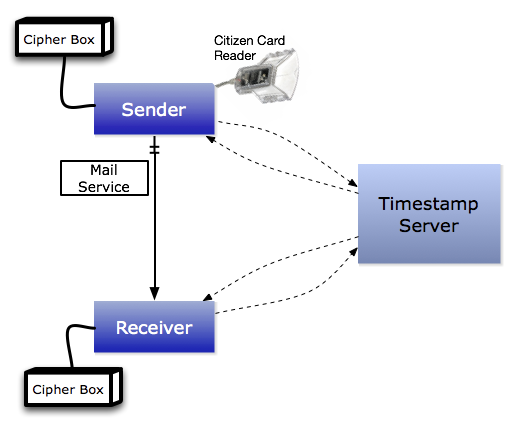
\includegraphics[width=12cm]{./Figures/chart.png}
\caption{Arquitectura do Sistema}
\label{fig:chart}
\end{figure}

O Sender terá que ter uma Caixa de Cifra e o adaptador do Cartão de Cidadão e respectivo Cartão ligados ao seu PC.
A primeira operação a ser executada, logo depois do zip, é a assinatura da mensagem. Para isso recorre ao seu Cartão de Cidadão e ao Certificado de Autenticação que se encontra dentro do mesmo.
Depois de a mensagem estar assinada, a segunda operação a ser executada é a validação por timestamp. Tal como assinalado na figura \textbf{Figura~\ref{fig:chart}}, o Sender envia um pedido ao Servidor de Timestamps e recebe um Timestamp seguro para juntar à sua mensagem: os detalhes desta operação serão explicados na Secção~\ref{section:timestamp}.
Finalmente, a última operação a ser executada é a cifra com a Caixa de Cifra que foi fornecida pelo Cliente que requeriu este trabalho.
Quando o Receiver recebe a mensagem protegida efectua as operações pela ordem inversa, começando pela decifra, verifica a validade do Timestamp através do servidor e, finalmente, verifica a Assinatura (fazendo sempre depois o unzip).

\section{Zipping/Unzipping}
Sempre que o Sender envia uma mensagem esta é, em primeiro lugar, zipada. 
O zip é efectuado em um ou mais ficheiros através da selecção da pasta com os dados a enviar, para isso é criado um Array com os ficheiros contidos na pasta, que são depois zipados.
O output da operação de zip é um único ficheiro comprimido.
A operação de unzip é feita de forma inversa.
Para efectuar a operação, quer de zip quer de unzip, foi utilizada a biblioteca \textit{zip} nativa no Java 6.

\section{Sign/Verify}
A segunda operação a ser executada pelo Sender é a operação de Assinatura; no caso do Receiver esta é a penultima última operação a ser executada (antes do unzip).
Para assinar/validar os ficheiros é utilizado o Cartão do Cidadão e a lib pkcs11.
É utilizado o Certificado de Autenticação presente no cartão e a mensagem é assinada com a respectiva chave privada. Juntamente com a mensagem assinada é também enviado o Certificado com a chave pública.

Do lado do Receiver, para este verificar se a mensagem é valida, utiliza a chave pública que foi enviada através do certificado.

\section{Timestamp Seguro}
\label{section:timestamp}
Para utilizar um mecanismo de TImestamp seguro, o Sender envia ao Servidor de Timestamp um pedido com o hash do(s) ficheiro(s). Estre cria um Timestamp com a data actual e devolve para o Sender todos os dados cifrados com a sua chave pública, ou seja, assinados por este enquanto "CA".
A mensagem é assim retornada no seguinte formato:
Kp(H(m),T),T
Em que H(m) é a hash da mensagem, T o timestamp e Kp a chave pública do Servidor de Timestamp. 

O Receiver para verificar a validade do timestamp, ou seja, para assegurar que a mensagem foi mesmo enviada àquela hora, envia a mensagem assinada para o Servidor de Timestamp. A mensagem foi cifrada com a chave pública deste para que este possa ter a certeza que foi mesmo ele que a assinou. Para fazer a verificação utiliza, então, a sua chave privada.

\section{Cipher/Decipher}
A última operação a ser executada pelo Sender e a primeira a ser executada pelo Receiver é a operação de cifra (e decifra, respectivamente).
Para efectuar a cifra, o Sender utiliza a Caixa de Cifra ethernet fornecida pelo Cliente. A interface desta caixa é em C e para que o serviço interaja com esta foi utilizado o JNI.
A mensagem é cifrada por blocos, o que possibilita a cifra de ficheiros de tamanho elevado.

O Receiver utiliza também uma Caixa de Cifra ethernet para descifrar a mensagem, aplicando-se a utilização das mesmas bibliotecas.

\section{Base64}
Antes de salvar (ou enviar para o email) o ficheiro protegido é feito do lado do Sender a codificação para base64 de forma a garantir compatibilidade com vários protocolos e evitar envio de cabeçalhos pois permite a codificação de 8 bits de data em 6 bits de transmissão sendo assim compativel com a maioria dos serviços de email que utilizem o protocolo standard.

O receiver faz a descodificação de base64 mesmo antes de proceder à decifra da mensagem.


